The structure of a disoTPS on a square lattice is shown in Figure \figref{fig:disoTPS_structure}. It can be constructed in three steps. First, a square PEPS is rotated by $45^\circ$. Next, the orthogonality hypersurface is constructed as a column of auxiliary tensors. The auxiliary tensors are connected in a line similar to an MPS and placed between two columns of PEPS tensors. Note that, in contrast to the standard isoTPS, the tensors of the orthogonality hypersurface do not carry any physical degrees of freedom and only have virtual indices. Lastly, the isometry condition is enforced such that all arrows point towards the orthogonality hypersurface. Tensors left of the orthogonality hypersurface are thus brought into a left-isometric form and tensors right of the orthogonality hypersurface are brought into a right-isometric form, as shown in Figure \figref{fig:disoTPS_structure}. The auxiliary tensors making up the orthogonality hypersurface are isometrized such that all arrows point towards a single auxiliary tensor, the orthogonality center. We further impose that the quantum state represented by the disoTPS is normalized to one. Because of the isometry condition, this reduces to the constraint that the orthogonality center must be a tensor of norm one.\par
\begin{figure}[ht]
	\centering
	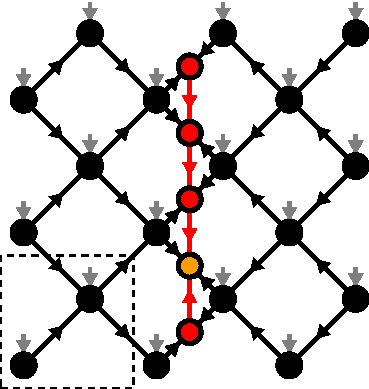
\includegraphics[scale=1]{figures/tikz/disoTPS/disoTPS_structure/disoTPS_structure.pdf}
	\caption{A diagonal isometric tensor network on a $3\times3$ diagonal square lattice is constructed from site tensors $T_j$ (drawn in black) and an orthogonality hypersurface of auxiliary tensors $W_j$ (drawn in red). The orthogonality hypersurface is rotated by $45^\circ$ with respect to the lattice. The dashed lines denote a single unit cell. The single tensor in the orthogonality hypersurface with only incoming arrows is called the orthogonality center (drawn in orange).}
	\label{fig:disoTPS_structure}
\end{figure}
In the following, we will denote the auxiliary tensors by $W_j$, and the tensors carrying physical degrees of freedom with $T_j$. The bonds connecting two $T$-tensors or a $T$-tensor and a $W$-tensor are truncated to a maximal bond dimension of $D$, while the maximal bond dimension between two $W$-tensors is denoted as $\chi$. Similar to isoTPS it is found that setting $\chi=f\cdot D$ with an integer $f\ge1$ produces good results in practice. We denote the dimension of the physical indices by $d$ in analogy to MPS and isoTPS. \par
Similar to isoTPS, the orthogonality center can easily and exactly be moved along the orthogonality hypersurface using QR-decompositions, compare Figure \figref{fig:isoTPS_moving_ortho_center}. Moving the orthogonality hypersurface to the left or to the right is a harder problem and will be discussed in Section \ref{sec:disoTPS_yang_baxter_move}. \par
\begin{figure}
	\centering
	% Store largest image in a box
	\savebox{\largestimage}{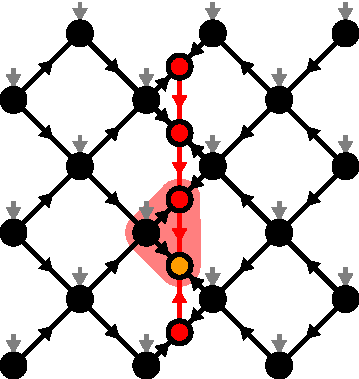
\includegraphics[scale=1]{figures/tikz/disoTPS/one_site_expectation_value/one_site_expectation_value_a.pdf}}
	\subcaptionbox{\label{fig:disoTPS_onesite_expectation_value_environment}}
	{%
		\usebox{\largestimage}
	}
	\quad\quad
	\subcaptionbox{\label{fig:disoTPS_onesite_expectation_value_computation}}
	{%
		\raisebox{\dimexpr.5\ht\largestimagea-.5\height}
		{%
			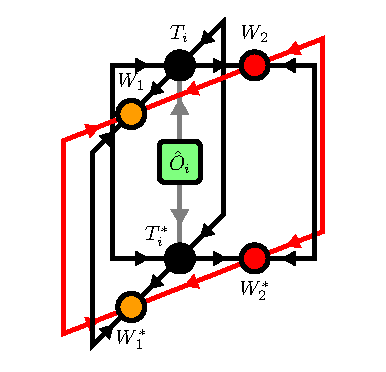
\includegraphics[scale=1.0]{figures/tikz/disoTPS/one_site_expectation_value/one_site_expectation_value_b.pdf}
		}
	}
	\caption{(a) The one-site wave function around a site $i$ is the sub network containing the site tensor $T_i$ and the two connected auxiliary tensors. (b) The computation of a single site expectation value reduces to the shown contraction over the one-site wave function, its complex conjugate, and the one-site operator $\hat{O}_i$.}
	\label{fig:disoTPS_onesite_expectation_value}
\end{figure}
Similar to MPS and isoTPS, disoTPS allow for the fast computation of expectation values of local operators. The expectation value $\bra{\Psi}\hat{O}_i\ket{\Psi}$ of a one-site operator $\hat{O}_i$ acting on site $i$ can be computed as follows: First, the orthogonality center is moved next to site $i$. We then define the \textit{one-site wave function} as the sub-network containing the site tensor $T_i$ and the two connected $W$-tensors. Note that the one-site wave function is connected to its environment only by bonds with incoming arrows. Next the wave function is contracted with its complex conjugate, sandwiching the operator $\hat{O}_i$ between the two. Due to the isometry condition, this reduces to a contraction of only the one-site wave function, its complex conjugate, and the operator $\hat{O}_i$, as shown in Figure \figref{fig:disoTPS_onesite_expectation_value}. This contraction has a computational cost scaling as $\mathcal{O}\left(\chi^3 D^3 + D^6d^2\right) = \mathcal{O}(D^6)$ and gives as result the desired expectation value. \par
\begin{figure}
	\centering
	% Store largest image in a box
	\savebox{\largestimage}{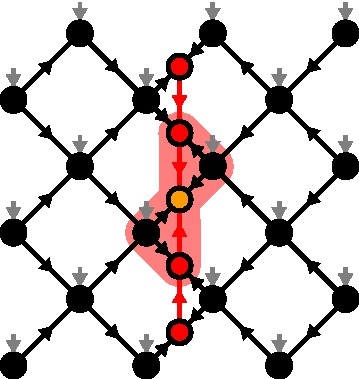
\includegraphics[scale=1]{figures/tikz/disoTPS/two_site_expectation_value/two_site_expectation_value_a.pdf}}
	\subcaptionbox{\label{fig:disoTPS_twosite_expectation_value_environment}}
	{%
		\usebox{\largestimage}
	}
	\quad\quad
	\subcaptionbox{\label{fig:disoTPS_twosite_expectation_value_computation}}
	{%
		\raisebox{\dimexpr.5\ht\largestimage-.5\height}
		{%
			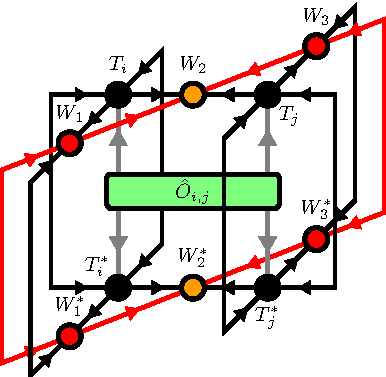
\includegraphics[scale=1.0]{figures/tikz/disoTPS/two_site_expectation_value/two_site_expectation_value_b.pdf}
		}
	}
	\caption{(a) The two-site wave function around neighbouring sites $i$ and $j$ is the sub network containing the site tensors $T_i$ and $T_j$ and the three connected auxiliary tensors. (b) The computation of a two-site expectation value reduces to the shown contraction over the two-site wave function, its complex conjugate, and the two-site operator $\hat{O}_{i,j}$.}
	\label{fig:disoTPS_twosite_expectation_value}
\end{figure}
The expectation value $\bra{\Psi}\hat{O}_{i,j}\ket{\Psi}$ of a two-site bond operator $\hat{O}_{i,j}$ acting on two neighbouring sites $i$ and $j$ can be computed similarly. First, the orthogonality center is moved such that it sits in the middle of the bond connecting sites $i$ and $j$. The \textit{two-site wave function} is then defined as the subnetwork containing the two site tensors $T_i$ and $T_j$ and three $W$-tensors as shown in Figure \figref{fig:disoTPS_twosite_expectation_value}, such that again all legs connecting the subnetwork to its environment are only decorated with arrows pointing towards the two-site wave function. The computation of the expectation value then reduces to the contraction of only the two-site wave function with its complex conjugate and the bond operator $\hat{O}_{i,j}$. The computational cost of this contraction scales as $\mathcal{O}\left(\chi^3D^3d^2\right) = \mathcal{O}(D^6)$.